\documentclass{beamer}
\usetheme{Boadilla}
\usecolortheme{sidebartab}

\usepackage{hyperref}
\usepackage{showexpl} 
\usepackage{graphicx}
\usepackage{color}
\usepackage{siunitx}
\usepackage[version=3]{mhchem}
\usepackage{chemfig}

\lstloadlanguages{[LaTeX]Tex} 
\lstset{% 
     basicstyle=\ttfamily\large, 
     commentstyle=\itshape\ttfamily, 
     showspaces=false, 
     showstringspaces=false, 
     breaklines=true, 
     breakautoindent=false, 
     captionpos=t,
     explpreset={numbers=none},
     pos=b
} 

\title{Introduction to writing with LaTeX}
\author{Markus Stocker}
\date{May 12, 2017}

\begin{document}
\maketitle

\begin{frame}
  \frametitle{Outline}
  
  \begin{itemize}
  \item Morning lecture
  \begin{itemize}
  \item What is \LaTeX
  \item Motivating \LaTeX 
  \item \LaTeX~software environment
  \item Basics of writing \LaTeX~documents
  \item Scientific documents with journal \LaTeX~templates
  \item \LaTeX~for slides and posters
  \item Collaborative writing and versioning of \LaTeX~documents
  \end{itemize}
  \item Afternoon hands-on
  \begin{itemize}
  \item Develop your \LaTeX~manuscript
  \item Style your manuscript with journal templates
  \item Revise your manuscript with track changes
  \item Create slides and a poster to present your work
  \item Collaborative writing with your co-authors
  \end{itemize}
  \end{itemize}
\end{frame}

\begin{frame}
  \frametitle{Schedule}
  
  \begin{center}
  \begin{tabular}{ll}
  10.00 - 11.30 & Lecture \\
  11.30 - 12.30 & \emph{Lunch} \\
  12.30 - 13.15 & Hands-on I \\
  13.15 - 13.30 & \emph{Break} \\
  13.30 - 14.15 & Hands-on II \\
  14.15 - 14.45 & \emph{Coffee break} \\
  14.45 - 15.30 & Hands-on III \\
  15.30 - 15.45 & \emph{Break} \\
  15.45 - 16.30 & Hands-on IV \\
  16.30 - 17.00 & Closing
  \end{tabular}
  \end{center}
\end{frame}

\begin{frame}
  \frametitle{About me}
  
  \begin{itemize}
  \item Postdoc with PANGAEA at MARUM
  \item PhD in environmental informatics at University of Eastern Finland
  \item MSc in informatics at University of Zurich
  \item MSc in environmental science at University of Eastern Finland \emph{(soon)}
  \item My history with \LaTeX~goes back to 2001 when ...
  \end{itemize}
\end{frame}

\begin{frame}
  \frametitle{What is \LaTeX}
  
  \begin{itemize}
  \item Document preparation system
  \item Authored by Leslie Lamport, first released in 1985
  \item Most often used for technical or scientific documents
  \item Separate presentation from content
  \item Worry less about style and more about content
  \item Write plain text rather than formatted text
  \item Leave document design to designers
  \item Free software
  \item Available for Windows, Mac OS, Linux, Online
  \end{itemize}
  
  \begin{flushright}
  \url{https://www.latex-project.org}
  \end{flushright}
\end{frame}


\begin{frame}[fragile]
  \frametitle{What is \LaTeX}
	
  \begin{itemize}
  \item \textbf{Markup tagging} is central to writing with \LaTeX
  \item Label parts of the document using tags, e.g. \lstinline!\textit{}!
  \item It is used to do things like
  \begin{itemize}
  \item Define document structure, e.g. chapters, sections
  \item Style text, e.g. italic, symbols, tables
  \item Cite, footnote, cross-reference, ...
  \end{itemize}
  \item Anyone familiar with HTML?
  \end{itemize}
\end{frame}

\frame[containsverbatim]{ 
  \frametitle{Markup tagging}
		
  \begin{LTXexample}
\textit{Example} 
markup 
\underline{tagging}
  \end{LTXexample}
}

\frame[containsverbatim]{ 
  \frametitle{Markup tagging}
	
  \begin{LTXexample}
\begin{itemize}
\item Eggs
\item Milk
\item Cheese
\item Carrots
\end{itemize}
  \end{LTXexample}
}

\frame[containsverbatim]{ 
  \frametitle{Markup tagging}
	
  \begin{LTXexample}
$ E = mc^2 $
  \end{LTXexample}
}

\begin{frame}
  \frametitle{Why \LaTeX: Advantages}
  
  \begin{itemize}
    \item High typographic quality
    \item Excels at difficult typesetting tasks, e.g. mathematical text
    \item Makes things easy, e.g. citation, cross-reference, table of content
    \item Great engineering, fast and stable
    \item Even with long and complex documents
    \item No corrupt files, content loss, etc.
    \item Truly portable across systems
  \end{itemize}
\end{frame}

\begin{frame}
  \frametitle{Why \emph{not} \LaTeX: Disadvantages}
	
  \begin{itemize}
    \item Learning curve, somewhat difficult to learn
    \item Though, basics are \emph{really} easy
    \item Surely requires some time
    \item Not WYSIWYG
    \item More difficult in collaborative writing
    \item Less support for tracking changes
  \end{itemize}
\end{frame}

\begin{frame}
  \frametitle{Working with \LaTeX}
	
  \begin{itemize}
    \item You need a distribution
    \begin{itemize}
      \item Most likely TeX Live (\url{http://www.tug.org/texlive/})
      \item Or MiKTeX on Windows (\url{https://miktex.org/})
      \item Possibly MacTeX (\url{http://www.tug.org/mactex/})
    \end{itemize}
    \item Some kind of editor
    \item If you like Notepad, Vim, Emacs, ...
    \item Preferably,
    \begin{itemize}
      \item TeXstudio (\url{http://texstudio.org/})
      \item Texmaker (\url{http://www.xm1math.net/texmaker/})
      \item TeXnicCenter on Windows (\url{http://www.texniccenter.org/})
      \item TeXShop on Mac OS (\url{http://pages.uoregon.edu/koch/texshop/})
      \item Among others ...
    \end{itemize}
    \item Make use of packages, of which there are several thousands
  \end{itemize}
\end{frame}

\begin{frame}
  \frametitle{Working with \LaTeX}
  
  \begin{enumerate}
    \item Install distribution and editor
    \item Install required packages
    \item Write \LaTeX~document using editor
    \item Translate \LaTeX~document into PDF document
    \item Iterate over points (2) and 3-4 until done
  \end{enumerate}
\end{frame}

\begin{frame}
  \frametitle{TeXstudio}
  
  \begin{center}
    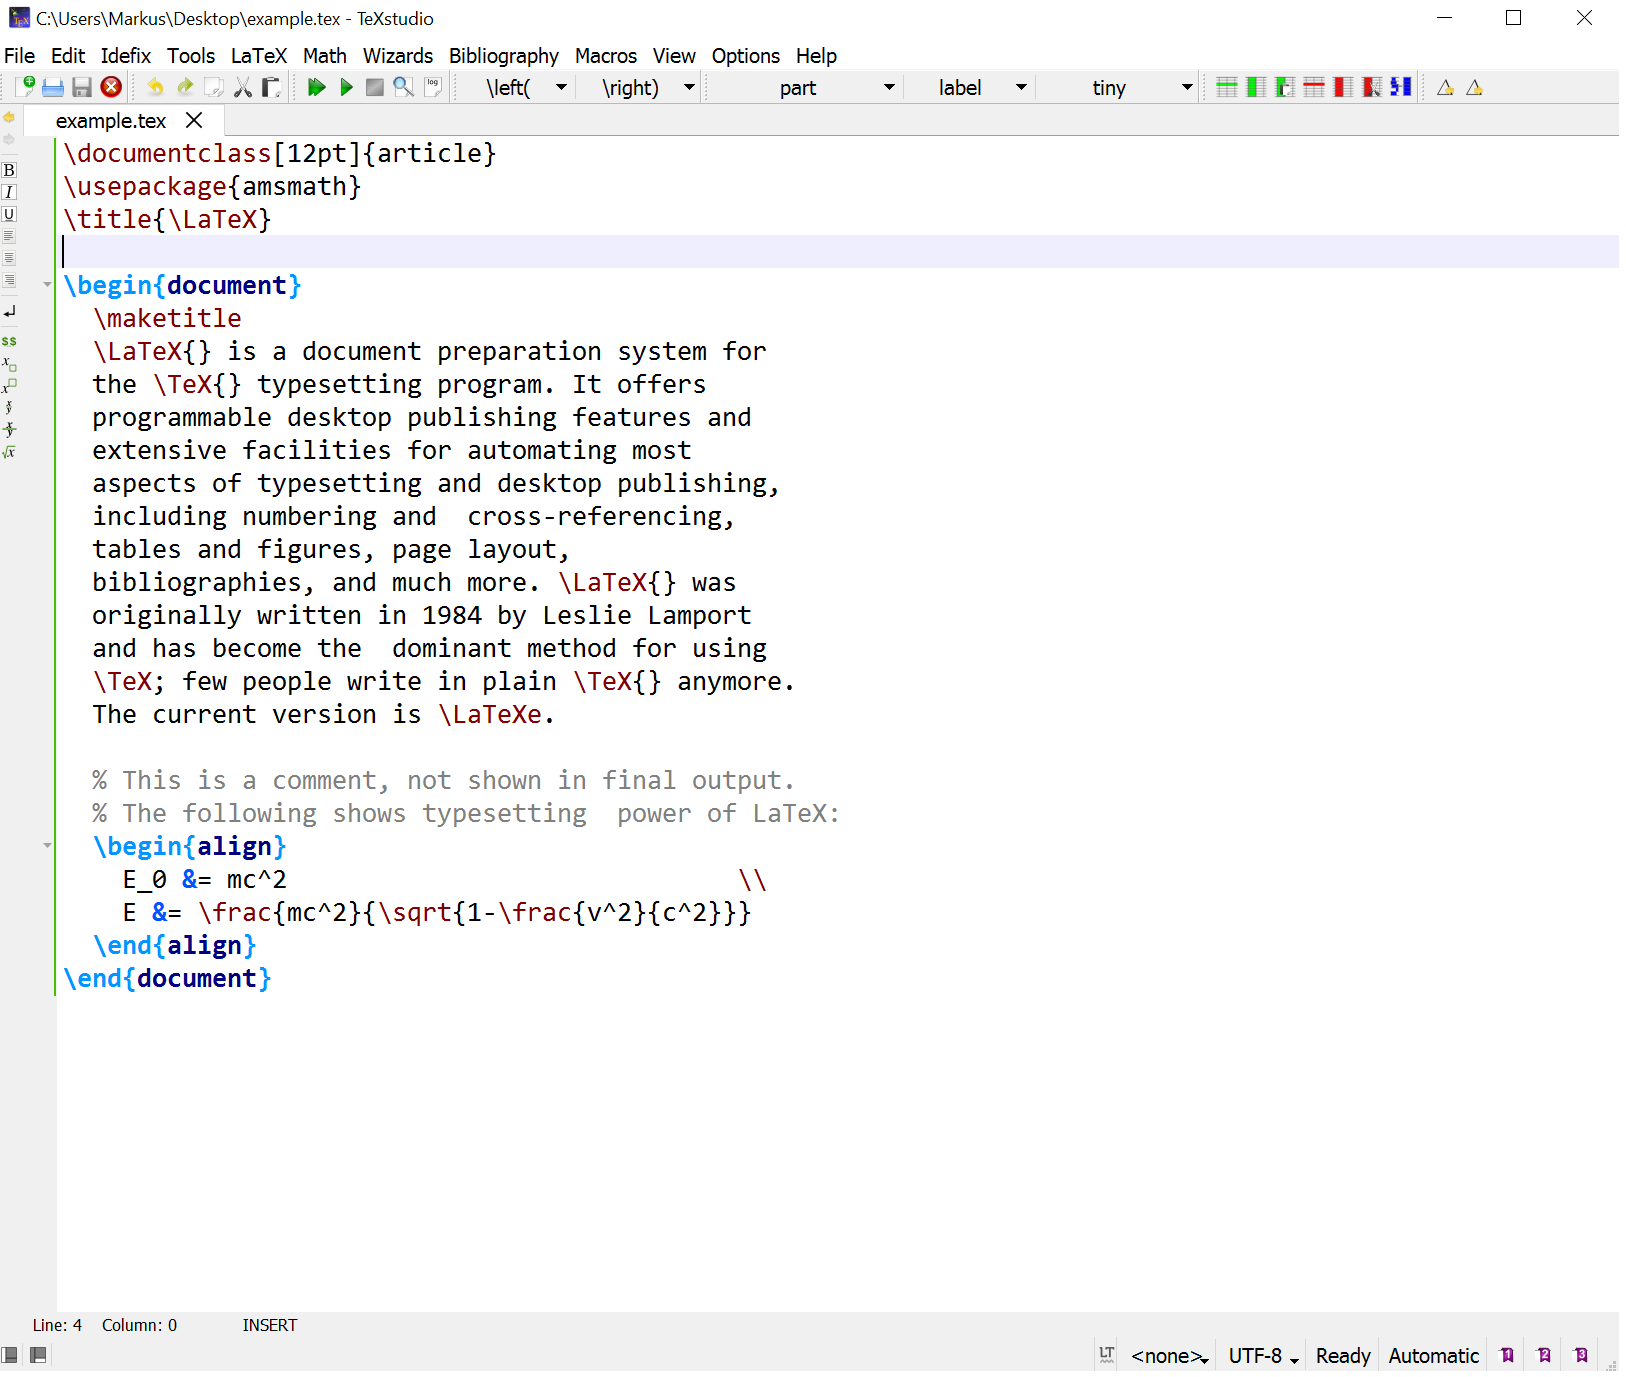
\includegraphics[height=0.8\textheight]{figures/texstudio.png}
  \end{center}
\end{frame}

\begin{frame}
  \frametitle{Writing \LaTeX~documents}
  
  \begin{itemize}
    \item Start with minimal document
    \item Develop it gradually by introducing new elements
    \item Structural elements, e.g. title, sections
    \item Style text, e.g. font size, italic, bold
    \item Mathematical and chemical formulae, quantities and units
    \item Tables and figures
    \item Cross-references, footnotes, and index
    \item Citation and reference list
    \item Table of contents, list of figures and tables
    \item Track changes
  \end{itemize}
\end{frame}

\frame[containsverbatim]{
  \frametitle{Minimal document}
 
  \begin{verbatim}
  \documentclass{article}
  
  \begin{document}
    Hello World.
  \end{document}
  \end{verbatim}
}

\begin{frame}
  \frametitle{Minimal document}
  
  \begin{center}
    
\includegraphics[width=0.3\textwidth]{figures/minimal.pdf}
  \end{center}
\end{frame}

\frame[containsverbatim]{
  \frametitle{Minimal document}
  
  \begin{verbatim}
  \documentclass{article}
  
  % I am a comment
  % This area is called the PREAMBLE
  % Used to load packages and configure your document
  
  \begin{document}
  
  % This is the BODY of the document
  % Document content goes here
  
  \end{document}
  \end{verbatim}
}

\frame[containsverbatim]{
  \frametitle{Article title}
  
  \begin{verbatim}
  \documentclass{article}
 
  \title{Shine On You Crazy Diamond}
  \author{Pink Floyd}
  \date{1975}
  
  \begin{document}
    \maketitle % Don't worry how it is displayed
               % It will look pretty good
  \end{document}
  \end{verbatim}
}

\begin{frame}
  \frametitle{Article title}
  
  \begin{center}
    
\includegraphics[width=0.8\textwidth]{figures/maketitle.pdf}
  \end{center}
\end{frame}


\frame[containsverbatim]{
  \frametitle{Article sections}
  
  \begin{verbatim}
  \documentclass{article}
  
  \title{Shine On You Crazy Diamond}
  \author{Pink Floyd}
  \date{1975}
  
  \begin{document}
    \maketitle
    
    \section{Introduction}
    \section{History}
    \section{Lyrics}
  
  \end{document}
  \end{verbatim}
}

\begin{frame}
  \frametitle{Article sections}
  
  \begin{center}
    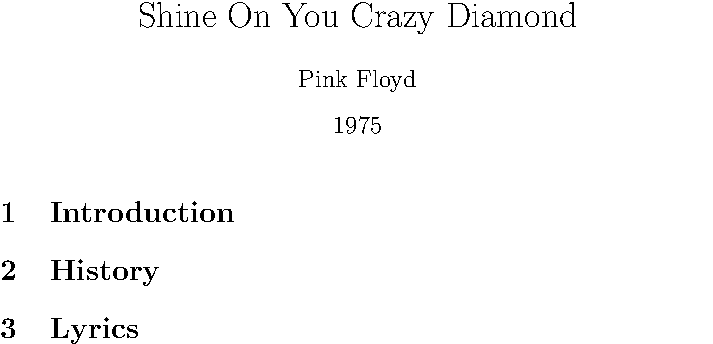
\includegraphics[width=0.8\textwidth]{figures/sections.pdf}
  \end{center}
\end{frame}

\frame[containsverbatim]{
  \frametitle{Sectioning}
  
  \begin{verbatim}
  % For article document class
  \section{...}
  \subsection{...}
  \subsubsection{...}
  \paragraph{...}
  \subparagraph{...}
  
  % Addtionally for book document class
  \chapter{...}
  \end{verbatim}
}

\frame[containsverbatim]{ 
  \frametitle{Text styling}
  
  \begin{LTXexample}
Remember \textbf{when} you \textit{were} young \underline{you} shone \texttt{like} the sun.

{\color{red}Now there's}     {\Huge{a}}       \textbf{\underline{look in} your}          eyes, like     {\tiny{``black holes       {\Large{in the sky}}.''}}
  \end{LTXexample}
}

\frame[containsverbatim]{ 
  \frametitle{Mathematical formulae}
  
  \begin{LTXexample}
\begin{displaymath}
  \lim_{n \to \infty} 
  \sum_{k=1}^n \frac{1}{k^2}
\end{displaymath}

Math $a^2 + b^2 = c^2$ in text style.
  \end{LTXexample}
}

\frame[containsverbatim]{ 
  \frametitle{Chemical formulae}
  
  \begin{LTXexample}
\ce{CO2}

\ce{CO2 + C -> 2 CO}

This is a \ce{H2O} molecule.

I can do charges \ce{CrO4^2-} and much more.
  \end{LTXexample}
}

\frame[containsverbatim]{ 
  \frametitle{Chemical formulae}
  
  \begin{LTXexample}
\chemfig{A*6(-B=C(-CH_3)-D-E-F(=G)=)}
  \end{LTXexample}
}

\frame[containsverbatim]{ 
  \frametitle{Quantities and units}
  
  \begin{LTXexample}
\num{.3e45}

\numlist{10;30;50;70}

\numrange{10}{30}

\si{\kilo\gram\metre\per\square\second}

\SI{1.25}{\metre\per\second}
  \end{LTXexample}
}

\end{document}

% TODO: Describe JabRef
% Resources
% - https://tobi.oetiker.ch/lshort/lshort.pdf
% - https://de.sharelatex.com/learn/Chemistry_formulae
